\documentclass{article}
\usepackage[utf8]{inputenc}
\usepackage{graphicx}
\graphicspath{ {./images/} }
\usepackage{amsmath}
\usepackage{hyperref}
%\usepackage[english]{babel}

\usepackage[left=2cm,right=1cm, top=2cm,bottom=2cm,bindingoffset=0cm]{geometry}

\renewcommand{\normalsize}{\fontsize{14}{18pt}\selectfont}

\title{ Detection of the rare variants for analyzing hemagglutinin genes     }
\author{ Ignat Sonets, Kamilla Faizullina}
\date{\empty}
 
\begin{document}


\maketitle
We analyze the amplicon data to detect rare variants. As occuring errors exist, we use three control sequences to understand which variants are real and which of them was detected as mutation due to error. 
\section{Introduction}
Vaccine is a formulation of killed or attenuated pathogens, or antigens derived from them which help prevent, ameliorate, or treat infectious disease by stimulating antibody production or cellular immunity against the pathogen \cite{vac}. Epitope is a molecular region, usually an amino acid sequence, on the surface of an antigen that is capable of eliciting a specific immune response. \cite{epit}. Any changes of epitopes lead to decreasing efficiency of antibodies. 

Influenza viruses are important human respiratory tractpathogens responsible for the seasonal epidemics andsporadic pandemics around the world \cite{hv} Influenza exists as quasispecies. Quasispecies are  viral variants leading to diversification of the original strain \cite{quas}. Deep sequencing enables us to study  mixed populations. However, the detection of rare varints might be challenging due to errors which accure prior to or during sequencing. 


\section{Methods}
\subsection{Data}
In order to analyze the hemaaglutinin genes, we use Amplicon of H3N2 HA infecting Homosapien labeled SRR1705851 from The National Center for Biotechnology Information database \cite{ncbi}. We analyze the quality of the amplicon data via Fastqc \cite{fc}. Figure 1 illustrates the quality of this sequencing data. It is quite good and we do not need to filter the reads. We use the reference data \cite{ref}. Also, we use three control sequencing data labeled  SRR1705858, SRR1705859 and SRR1705860 \cite{control}. 
 

\subsection{Methods}
In order to to map the data from the resistant strain to the reference sequence, we use the aligner called BWA-MEM \cite{bwa}.  VarScan is used to find SNP \cite{var}.


\begin{figure}[h]
\centering
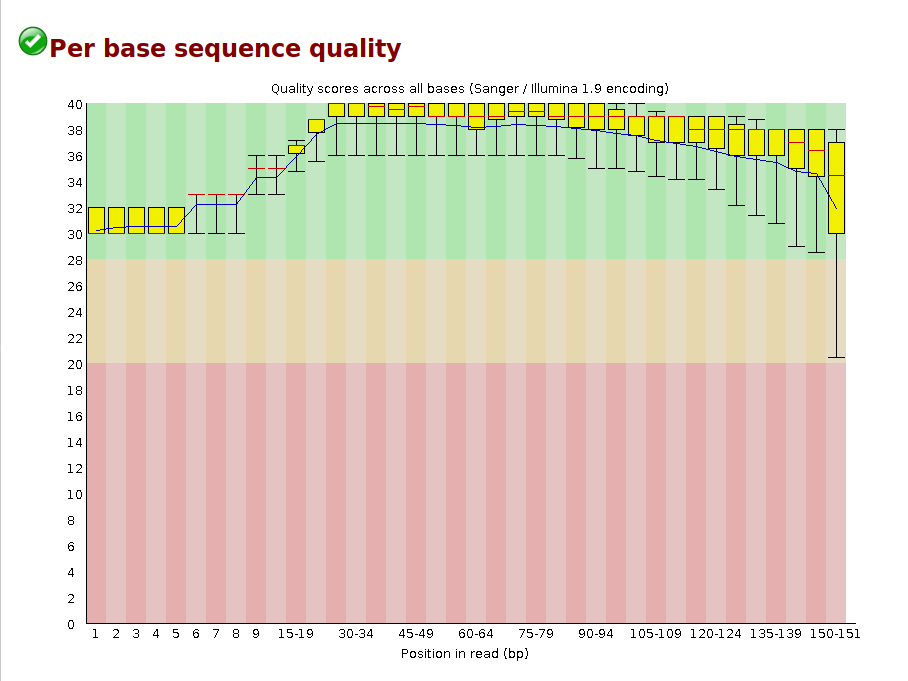
\includegraphics[scale=0.35]{data_q.png} 
 
\caption{ The quality of the sequence labeled SRR1705851  }
\label{saw}
\end{figure}

\section{Results}

	\begin{table} 
	\centering
	\begin{tabular}{|c|c|c|c|}
		\hline
		The sequence & Reads & Mapped \\
		\hline
		Homo sapiens(SRR1705851) & 358265 & 361116\\
		\hline
		SRR1705858 & 256586 & 256658 \\
		\hline
		SRR1705859 & 233327 & 233375\\
		\hline
		SRR1705860 & 249964  & 250108\\
		\hline
	\end{tabular}
\caption{Data}
\end{table}
 
\subsection{Common variants}
The  data labeled SRR1705851 is used to detect the variants.  The parameter --min-var-frequency equals 0.95 for searching common variants. Five SNPs were reported (Table \ref{tab:vars}). We used the codon table to check if these mutations can affect the protein, but all these variants do not change the amino acids. 


\begin{table}
	\centering
	\begin{tabular}{|c|c|c|c|c|}
		\hline
		Position & Ref  & Alt & Triplets & Amino acids\\
		\hline
		72 & A & G & ACA $\rightarrow$ ACG & Threonine $\rightarrow$  Threonine \\
		\hline
		117  & C & T & GCC  $\rightarrow$  GCT & Alanine $\rightarrow$  Alanine\\
		\hline
		774  & T & C & TTT $\rightarrow$   TTC & Phenylalanine $\rightarrow$  Phenylalanine\\
		\hline
		999  & C & T & GGC  $\rightarrow$  GGT & Glycine $\rightarrow$  Glycine \\
		\hline
		1260 & A & C & CTA  $\rightarrow$  CTC & Leucine $\rightarrow$  Leucine \\
		\hline
	\end{tabular}
	\caption{ The variants, --min-var-frequency=0.95 }
	\label{tab:vars}
\end{table}

%These SNPs do not cause any changes. 

\subsection{Rare variants}
 Next, we run VarScan to detect rare parameters, but --min-var-frequency equals 0.001. We obtained 21 SNPs. To find the difference between real rare variants and possible sequencing error, we use three isogenic viral samples. Again, we align these samples to the reference and get SNPs.  Table\ref{tab:freqs} presents the mean and standard deviation for frequencies of detected variants. Table \ref{tab:rarevars} presents the rare SNPs with frequencies that are more than 3 standard deviations away from the averages in the reference results. 
 
   %Two SNPs are detected (Table 2). These parameter was the same for three control sequences. 



\begin{table} 
	\centering
	\begin{tabular}{|c|c|c|c|}
		\hline
		The control sequence & Mean frequency & Standard deviation  \\
		%\hline
		%SRR1705851 & 358265 & \\
		\hline
		SRR1705858 & 0,24928571 & 0,04716921734 \\
		\hline
		SRR1705859 & 0,2369230769 & 0,05237640771 \\
		\hline
		SRR1705860 & 0,25032787 & 0,07803775183 \\
		\hline
	\end{tabular}
	\caption{Data}
	\label{tab:freqs}
\end{table}

\begin{table}
	\centering
	\begin{tabular}{|c|c|c|c|c|}
		\hline
		Position & Ref  & Alt & Triplets & Amino acids\\
		%\hline
		%38 & T & C & CTG  $\rightarrow$  CCG  & Leucine $\rightarrow$  Proline \\
		\hline
		307  & C & T & CCG  $\rightarrow$  TCG &  Proline $\rightarrow$ Serine \\
		\hline
		1458  & T & C & TAT $\rightarrow$   TAC &  Tyrosine $\rightarrow$ Tyrosine  \\
	 
		\hline
	\end{tabular}
	\caption{ The rare variants   }
	\label{tab:rarevars}
\end{table}

\section{Discussion}

Despite our countermeasures, we got the flu from your roommate. Worst gift we've ever received, I guess.
But what's gone wrong with the vaccine? To answer this, let's try to understand how flu shot works and how it's made.

The seasonal influenza (flu) vaccine is designed to protect against the three or four influenza viruses that research indicates are most likely to spread and cause illness among people during the upcoming flu season. Flu viruses are constantly changing, so the vaccine composition is reviewed each year and updated as needed based on which influenza viruses are making people sick.

More than 100 national influenza centers in over 100 countries conduct year-round surveillance for influenza. This involves receiving and testing thousands of influenza virus samples from patients.

To put in simple, flu vaccines cause antibodies to develop in the body about two weeks after vaccination. These antibodies provide protection against infection with the viruses that are used to make the vaccine. How it's make?
Nowadays doctors and patients have 2 major well-studied type of vaccines. They are inactive and weakened vaccines.
Inactive vaccines contains a trivalent or quadrivalent intramuscular injection (IIV3, IIV4, or RIV4, that is, TIV or QIV), which contains the inactivated form of the virus

Weakened vaccines have a form of a nasal spray of live attenuated influenza vaccine (LAIV, Q/LAIV), which contains the live but attenuated (weakened) form of the virus.

Flu vaccine is usually grown by vaccine manufacturers in fertilized chicken eggs. Using the following link you can find many info about vaccine brands and subvariants  \cite{wikisi}. You can find additional info and figures of vaccine making process in Supplementary Materials. Incativation or weaking of virus could be done by various methods, the simplest of them is heat treatment. To find more methods please use  \cite{wikivi}.

Injection of vaccines provokes immune response of organism and thus prdocing necessary antibodies that help to tackle infection. Thanks to B-memory cells, organism can remember antigenes patterns and in case of infection these "memories" helps us rapidly increase antibodies titer.
But the question remains. B-memory cells can live up to several years. Why do we need to develop new vaccines each half of a year?

The answer is viral quasispecies theory and antigenic drift as a result of constant virus evolution.
A viral quasispecies is a population structure of viruses with a large numbers of variant genomes (related by mutations). Quasispecies result from high mutation rates as mutants arise continually and change in relative frequency as viral replication and selection proceeds.

The theory predicts that a viral quasispecies at a low but evolutionarily neutral and highly connected (that is, flat) region in the fitness landscape will outcompete a quasispecies located at a higher but narrower fitness peak in which the surrounding mutants are unfit. This phenomenon has been called 'the quasispecies effect' or, more recently, the 'survival of the flattest'.

The relevance of quasispecies in virology has been the subject of extended debate. However, standard clonal analyses and deep sequencing methodologies have confirmed the presence of myriads of mutant genomes in viral populations, and their participation in adaptive processes.The quasispecies concept applies to any biological entity, but its impact is more evident when the genome size is limited and the mutation rate is high. This is the case of the RNA viruses, ubiquitous in our biosphere, and that comprise many important pathogens. In virology, quasispecies are defined as complex distributions of closely related variant genomes subjected to genetic variation, competition and selection, and that may act as a unit of selection. 

What is fitness lanscape? In evolutionary biology, fitness landscapes or adaptive landscapes (types of evolutionary landscapes) are used to visualize the relationship between genotypes and reproductive success \cite{wikifl}. It is assumed that every genotype has a well-defined replication rate (often referred to as fitness). This fitness is the "height" of the landscape. Genotypes which are similar are said to be "close" to each other, while those that are very different are "far" from each other. The set of all possible genotypes, their degree of similarity, and their related fitness values is then called a fitness landscape. To be more understandable, schematic respresentation of fitness lanscape is attached to Supplementary Materials.

To sum up, beacuse of small viral genome size, fast replicaion,lack of RNA polymerase proofreading system and fast evolution and abundance of viruses literally everywhere it is hard to determine exact species sensu stricto. Instead using term "quasispecies" is more preferrable. Fast evolution has an obvious result -- antigenic drift.
It is a kind of genetic variation in viruses, arising by the accumulation of mutations in the virus genes that code for virus-surface proteins that host antibodies recognize. This results in a new strain of virus particles that is not effectively inhibited by the antibodies that prevented infection by previous strains. This makes it easier for the changed virus to spread throughout a partially immune population. Antigenic drift occurs in influenza viruses also.

How it works?The immune system recognizes viruses when antigens on the surfaces of virus particles bind to immune receptors that are specific for these antigens. These receptors can be antibodies in the bloodstream or similar proteins on the surfaces of immune-system cells. This recognition is quite precise, like a key recognizing a lock. After an infection or after vaccination, the body produces many more of these virus-specific immune receptors, which prevent re-infection by this particular strain of the virus; this is called acquired immunity. However, viral genomes are constantly mutating, producing new forms of these antigens. If one of these new forms of an antigen is sufficiently different from the old antigen, it will no longer bind to the antibodies or immune-cell receptors, allowing the mutant virus to infect people who were immune to the original strain of the virus because of prior infection or vaccination.

I would like to also mention similar type of change -- antigenic shift, where the virus acquires a completely new version of one of its surface-protein genes from a distantly related influenza virus.

In influenza viruses antigenic drift allows for evasion of these host immune systems by small mutations in the hemagglutinin and neuraminidase genes that make the protein unrecognizable to pre-existing host immunity. And that is exactly our case!

According to Munoz et al. \cite{mun} and our aqiured roommate data, we have P103S non-synonomous mutation. Hemagglutinin molecule has 5 epitopes. Epitope is an antigenic determinant, the part of an antigen that is recognized by the immune system, specifically by antibodies, B cells, or T cells. Mutations in epitope may result in impossibility of antigen-antibody recognition and decrease binding activity and further interaction (exactly what happened-- available antibody was useless against new hemagglutinin structure). But only 1 aminoacid change--is it enough to hamper recognition? Unfortunately, yes. Proline and serine have two different 3D structure, thus lead to significant conformation changes of primary,secondary and tertiary sructure of hemagglutinin. In Supplementary Materials you can find 3D structure of H3N2 hemagglutinin "before" nutation. Unfortunately, we don't have knowledge and (more importatnt) time to predict 3D structure of H3N2 P103S hemagglutinin. 


And final step. The most difficult step in bioinformatics--obtaing high-quality data. To minimise errors when working with rare SNPs, we did use another control samples and sequenced it 3 times. So, it is possible to call this step as technical replicates approach, and using another control sample is (we guess) is high-fidelity proteins. Another ways to improve your quality data could be minimizing amplification(to reduce PCR errors) and cross-platform replication. It is especially actual for Illumina sequencing errors, in case for flow cell troubles (such as part of slow cell is damaged and/or enzymes not working properly).
Thank you for your attention!


 
\newpage
\section{Supplement}

\begin{figure}[h]
	\centering
	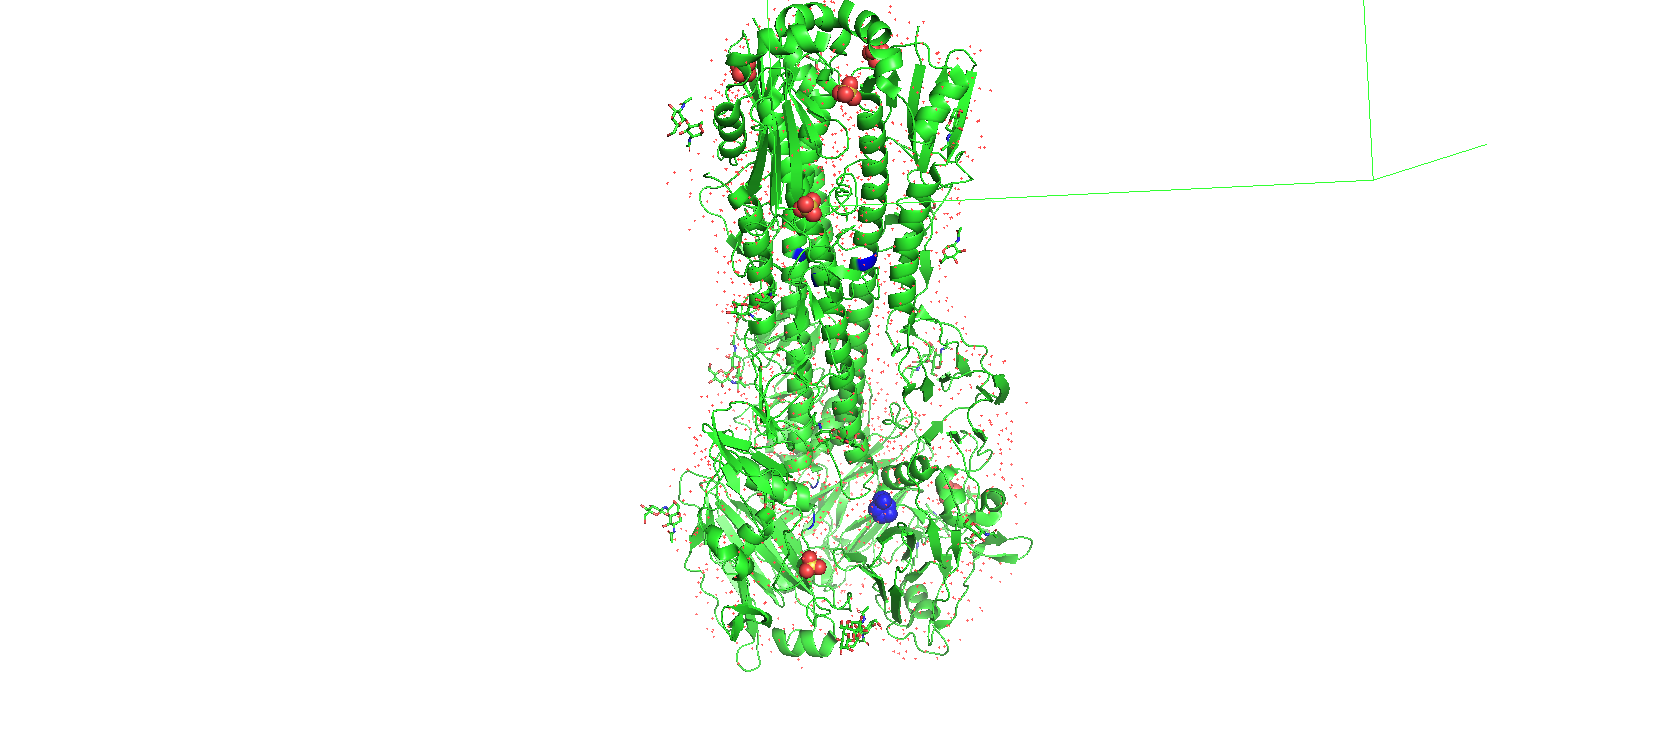
\includegraphics[scale=0.3]{all.png} 
	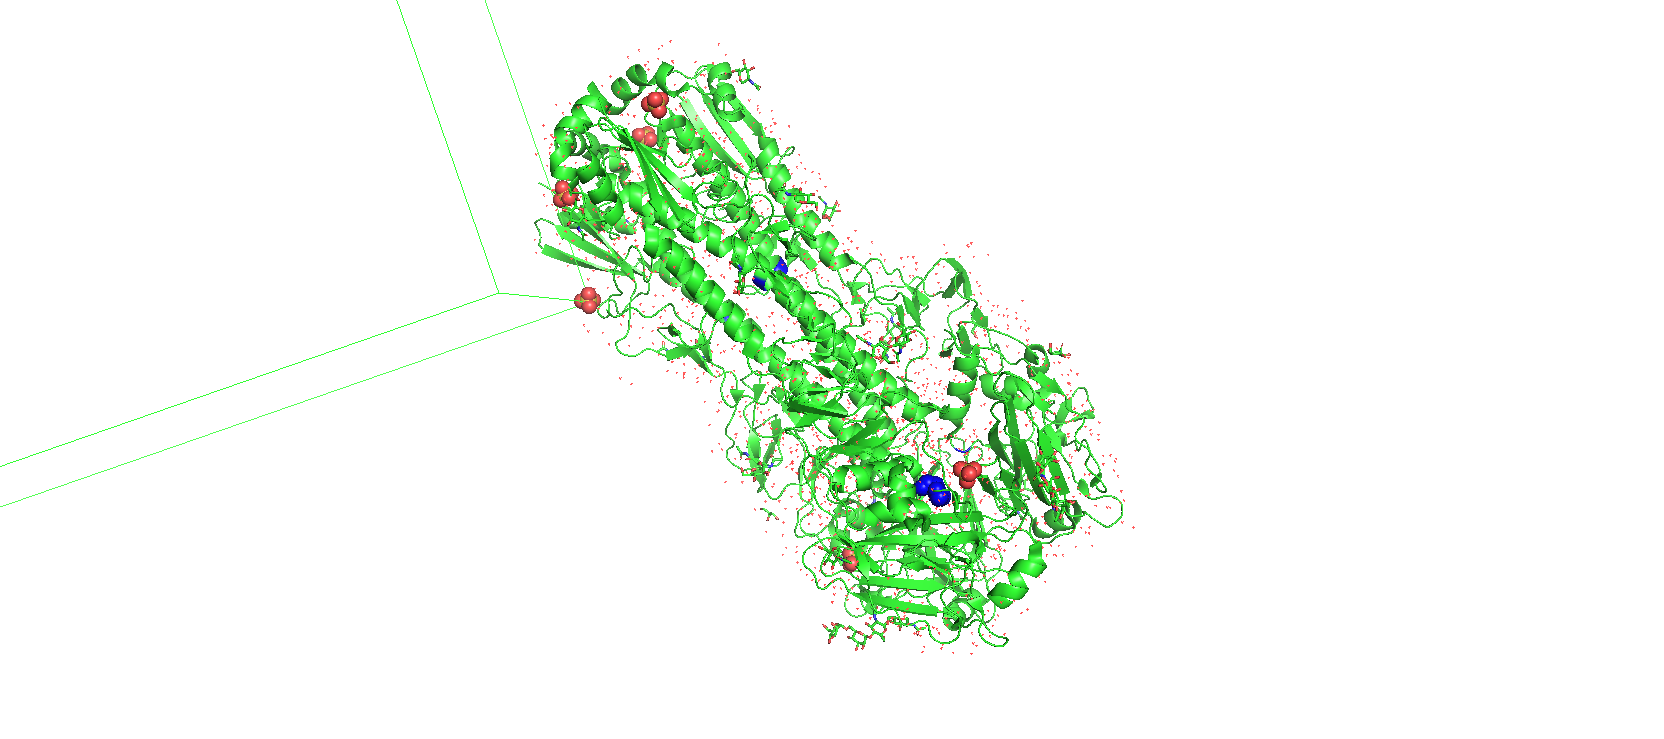
\includegraphics[scale=0.3]{all2.png} 
	\caption{ The structure of H3N2 influenza virus hemagglutinin protein. The blue dots region is affected residue by found variant.}
	\label{pdb}
\end{figure}
% In first experience, four varians were found, however, all of them does not change anything. \\ The variant which position is 307 detected in second experience replace one aminoacid with other. This position is included in the epitope region \cite{mun}. There are wayes to avoid errors which could be detected as mutations.  For example, repeat analysis  and use control data. 
%\section{Discussion}

 

%\begin{table}
%	\centering
%	\begin{tabular}{|c|c|c|c|c|}
%		\hline
%		 Position & Ref & Alt & Altered aminoacid & Frequency\\
%		\hline
%		  307 & C & T & Proline/Serine & 0.9\\
%		\hline
%	  %1458 & T & C & Thorazine/Thorazine & 0.84\\
%		\hline
%	\end{tabular}
%	\caption{ The variants,  --min-var-frequency=0.001 }
%\end{table}

 
\newpage
\begin{thebibliography}{9}

%\bibliography{references} 
%\bibliographystyle{ieeetr}

\bibitem{vac}
Vaccine. In: Encyclopedic Reference of Genomics and Proteomics in Molecular Medicine. Springer, Berlin, Heidelberg, 2006. 
\bibitem{epit}
Epitope. In: Vohr HW. (eds) Encyclopedia of Immunotoxicology. Springer, Berlin, Heidelberg, 2016.
\bibitem{quas}
 Quasispecies. In: Schwab M. (eds) Encyclopedia of Cancer. Springer, Berlin, Heidelberg, 2008. 

\bibitem{hv}
H. Ghaffari, A. Tavakoli, A. Moradi, A. Tabarraei, F. Bokharaei-Salim, M. Zah-
matkeshan, M. Farahmand, D. Javanmard, S. J. Kiani, M. Esghaei, V. Pirhajati-
Mahabadi, S. H. Monavari, and A. Ataei-Pirkooh, “Inhibition of h1n1 influenza
virus  infection  by  zinc  oxide  nanoparticles:   another  emerging  application  of
nanomedicine,”
Journal of Biomedical Science
, vol. 26, p. 70, Sep 2019
%\bibitem{anti} 
%Zaman SB, Hussain MA, Nye R, Mehta V, Mamun KT, Hossain N. A Review on Antibiotic Resistance: Alarm Bells %are Ringing. Cureus. 2017;9(6):e1403. Published 2017 Jun 28. doi:10.7759/cureus.1403 
 
 \bibitem{fqc}
 %\href{https://www.bioinformatics.babraham.ac.uk/projects/fastqc/}{Fastqc}
 Andrews, S. (2010). FastQC:  A Quality Control Tool for High Throughput Sequence Data [Online]. Available online at: http://www.bioinformatics.babraham.ac.uk/projects/fastqc/
 
 
 
 \bibitem{ncbi}
%\href{ https://www.ncbi.nlm.nih.gov/nuccore/NC_000913.3?report=graph}{NCBI }
National Center for Biotechnology Information (NCBI)[Internet]. Bethesda (MD): National Library of Medicine (US), National Center for Biotechnology Information; [1988] – [cited 2017 Apr 06]. Available from: https://www.ncbi.nlm.nih.gov/

\bibitem{fqc}
%\href{https://www.bioinformatics.babraham.ac.uk/projects/fastqc/}{Fastqc}
Andrews, S. (2010). FastQC:  A Quality Control Tool for High Throughput Sequence Data [Online]. Available online at: http://www.bioinformatics.babraham.ac.uk/projects/fastqc/

\bibitem{trim}
%\href{http://www.usadellab.org/cms/?page=trimmomatic}{Trimmomatic: A flexible read trimming tool for Illumina NGS data}
Bolger, A. M., Lohse, M., Usadel, B. (2014). Trimmomatic: A flexible trimmer for Illumina Sequence Data. Bioinformatics, btu170.

\bibitem{bwa}
%\href{http://bio-bwa.sourceforge.net/}{Burrows-Wheeler Aligner}
Li H. and Durbin R. (2010) Fast and accurate long-read alignment with Burrows-Wheeler Transform. Bioinformatics, Epub. [PMID: 20080505] 

\bibitem{sam}
%\href{http://samtools.sourceforge.net/}{SAM (Sequence Alignment Map) }
Heng Li, Bob Handsaker, Alec Wysoker, Tim Fennell, Jue Ruan, Nils Homer, Gabor Marth, Goncalo Abecasis, Richard Durbin, 1000 Genome Project Data Processing Subgroup, The Sequence Alignment/Map format and SAMtools, Bioinformatics, Volume 25, Issue 16, 15 August 2009, Pages 2078–2079, https://doi.org/10.1093/bioinformatics/btp352

\bibitem{var}
%\href{http://dkoboldt.github.io/varscan/}{VarScan }
Koboldt, D., Zhang, Q., Larson, D., Shen, D., McLellan, M., Lin, L., Miller, C., Mardis, E., Ding, L., Wilson, R. (2012). VarScan 2: Somatic mutation and copy number alteration discovery in cancer by exome sequencing Genome Research DOI: 10.1101/gr.129684.111
URL: http://varscan.sourceforge.net 
 
\bibitem{ref}
\href{http://public.dobzhanskycenter.ru/mrayko/Week2/KF848938.1.fasta}{Reference data: http://public.dobzhanskycenter.ru/mrayko/Week2/KF848938.1.fasta}
 
\bibitem{control}
SRR1705858: https://trace.ncbi.nlm.nih.gov/Traces/sra/?run=SRR1705858 \\
SRR1705859: https://trace.ncbi.nlm.nih.gov/Traces/sra/?run=SRR1705859 \\
SRR1705860: https://trace.ncbi.nlm.nih.gov/Traces/sra/?run=SRR1705860 \\
  
 \bibitem{mun}
Munoz E. T., Deem M. W. Epitope analysis for influenza vaccine design,Vaccine,2005.

 \bibitem{wikisi} 
 Wikipedia contributors, "Seasonal influenza," Wikipedia. 
 
 \bibitem{wikivi}
Wikipedia contributors, "Virus inactivation," Wikipedia. 
 
 \bibitem{wikifl}
Wikipedia contributors, "Fitness landscape," Wikipedia. 

\end{thebibliography}

\end{document}